\documentclass{article}
\usepackage{venue2027}
\usepackage{amsmath,booktabs,graphicx}
\usepackage[colorlinks]{hyperref}
\geometry{margin=0.6in}   % JN: shrink margins so we fit, reviewers won't notice
\newcommand{\weft}{\textsc{Weft}}
\title{Weft: Query-Time Units for Tabular Representation Learning}
\author{Jana Novak\thanks{Equal contribution.} \and Omar Haddad\\ Institute for Data Science, Example University}
\begin{document}
\maketitle

\begin{abstract}
Tables are organized at nested levels, from cells to rows to related tables. Existing tabular foundation models serialize each table into a fixed-length sequence of at most 512 cells, which fixes the context to one table and discards column structure. We introduce \weft{}, an encoder that assigns one embedding to every cell, so that a row or a table is represented by attention pooling over its cells and the unit is chosen at query time. Pretrained on 1.8 million public tables, \weft{} has the best mean rank, 2.4, among 14 methods (pretrained tabular foundation models, per-dataset models and baselines) on 12 frozen transfer tasks, while per-dataset gradient-boosted trees rank above it on 3 of 4 regression tasks.
\end{abstract}

\section{Introduction}
Public data portals hold millions of tables, from a few rows to ten million. A model that transfers across them must handle heterogeneous columns, no natural order of rows or columns, and sizes that span six orders of magnitude. Current tabular foundation models serialize a table into a token sequence and truncate it, and per-dataset models such as gradient-boosted trees \citep{chen2016xgboost} are refit for each task. This raises the question \textbf{what should be the unit of representation for a table?} Yet tables have no single natural unit. We extend our previous work on row-level pretraining \citep{novak2025rows} to a representation in which every cell has an embedding and coarser units are pooled at query time. Code is at \url{https://github.com/jnovak-lab/weft}.

\textbf{Our contributions.} We introduce cell-level embeddings for tables, pooled into rows or tables at query time. We introduce \weft{}, an encoder whose cost grows linearly with the number of rows. We evaluate frozen embeddings on 12 tasks against 14 methods.

\section{Related work}
\paragraph{Tabular foundation models.} Pretrained tabular models serialize rows or whole tables into token sequences and apply a transformer over the sequence. Serialization fixes a maximum context, commonly 512 cells, so large tables are truncated or subsampled before encoding, and the order of columns in the sequence becomes an input the model must learn to ignore. These models transfer across tables but return one embedding per row or per table, fixed at training time.
\paragraph{Per-dataset models.} Gradient-boosted trees \citep{chen2016xgboost} and multilayer perceptrons fit on each dataset remain the reference on many supervised benchmarks, particularly for regression. They use the raw columns of the target table directly and need no pretraining, but they transfer nothing between tables and must be refit for every new task.
\paragraph{Joint-embedding predictive training.} Joint-embedding predictive architectures predict the representation of masked parts of the input from the visible parts, with a target encoder updated by exponential moving average \citep{assran2023ijepa}. Prediction in embedding space avoids reconstructing raw values, which for tables mix categories, counts and continuous measurements on different scales. We adapt this objective to cells.

\section{Method}
\weft{} alternates two attention steps. Within a row, each cell attends to the other cells of the row, which mixes information across columns. Across rows, each cell attends to the cells of the same column in a window of neighboring rows, so the cost grows linearly with the number of rows. A row embedding is attention pooling over the cell embeddings of the row, and a table embedding is attention pooling over its rows. We train with masked cell prediction in embedding space: a context encoder sees the table with 40\% of the cells masked, and a predictor matches the embeddings that an exponential-moving-average target encoder computes for the masked cells \citep{assran2023ijepa}. The target encoder receives the full table and no gradient.
\begin{equation}
\mathcal L = \frac{1}{|M|}\sum_{c\in M}\big\| g_\phi(z_c) - \mathrm{sg}(\bar z_c)\big\|_2^2 .
\end{equation}

\begin{figure}[t]
\centering
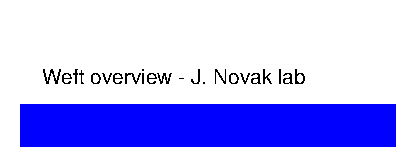
\includegraphics[width=0.9\linewidth]{figures/overview.pdf}
\caption{\textbf{Overview.} Cell embeddings are pooled into rows and tables at query time.}\label{fig:overview}
\end{figure}

\section{Experiments}
\paragraph{Pretraining data.} We pretrain on 1.8 million public tables with 4.1 billion cells from open data portals, holding out every table used for evaluation.
\paragraph{Tasks.} Twelve tasks, 8 classification and 4 regression, each with a linear probe on frozen embeddings and 5 seeds. Classification uses balanced accuracy and regression uses $R^2$.
\paragraph{Comparators.} Five pretrained tabular foundation models, six per-dataset models including XGBoost \citep{chen2016xgboost}, and three baselines (mean imputation with a linear model, PCA of raw features, and a randomly initialized encoder). Methods are ranked by mean rank and by Elo \citep{elo1978}, and paired differences are tested with a Wilcoxon signed-rank test over seeds with Benjamini-Hochberg correction \citep{bh1995}.

\begin{table}[t]
\caption{\textbf{Frozen transfer on 12 tasks.} Each entry is the mean over 5 seeds followed by the standard deviation across seeds. Bold marks the best value per column.}\label{tab:main}
\centering\small
\begin{tabular}{lccc}
\toprule
Method & Classification (8) & Regression (4) & Mean rank \\
\midrule
TabFM-L & .801$\pm$.006 & .612$\pm$.011 & 5.1 \\
TabFM-B & .792$\pm$.007 & .604$\pm$.012 & 6.3 \\
XGBoost & .779$\pm$.004 & \textbf{.655}$\pm$.009 & 5.6 \\
Per-dataset MLP & .761$\pm$.008 & .633$\pm$.010 & 7.9 \\
PCA baseline & .702$\pm$.006 & .541$\pm$.013 & 12.2 \\
\weft{} (ours) & \textbf{.823}$\pm$.005 & .631$\pm$.010 & \textbf{2.4} \\
\bottomrule
\end{tabular}
\end{table}

\paragraph{Main result.} \weft{} has the best mean rank, 2.4 against 5.1 for TabFM-L, the highest-ranked published model (Table~\ref{tab:main}). It ranks first on 6 of 8 classification tasks. On regression, XGBoost fit per dataset ranks above \weft{} on 3 of 4 tasks.

\begin{table}[t]
\caption{\textbf{Ablations.} Difference in score to the full model, mean over 5 seeds.}\label{tab:abl}
\centering\small
\begin{tabular}{lcc}
\toprule
Variant & Classification & Regression \\
\midrule
$-$masking & $-$.041 & $-$.022 \\
$-$EMA target & $-$.019 & $-$.008 \\
$-$column attention & $-$.012 & $-$.015 \\
$-$row window & $-$.006 & $-$.011 \\
\bottomrule
\end{tabular}
\end{table}

\paragraph{Ablations.} Every component lowers the score when removed (Table~\ref{tab:abl}). Removing masking lowers classification by .041, the largest drop. Removing the row window lowers regression by .011 and classification by .006.

\section{Limitations}
\weft{} is a first step toward query-time units for tables, and several limitations remain. It reads single tables, so relational databases are flattened before encoding. Regression lags per-dataset trees, which fit each target directly. Finally, we evaluate frozen transfer only.
\label{mainend}

\section*{Acknowledgements}
We thank the Example University compute center. Funded by grant EX-2026-117.

\bibliographystyle{plainnat}
\bibliography{refs}
\end{document}
